\documentclass[1p]{elsarticle_modified}
%\bibliographystyle{elsarticle-num}

%\usepackage[colorlinks]{hyperref}
%\usepackage{abbrmath_seonhwa} %\Abb, \Ascr, \Acal ,\Abf, \Afrak
\usepackage{amsfonts}
\usepackage{amssymb}
\usepackage{amsmath}
\usepackage{amsthm}
\usepackage{scalefnt}
\usepackage{amsbsy}
\usepackage{kotex}
\usepackage{caption}
\usepackage{subfig}
\usepackage{color}
\usepackage{graphicx}
\usepackage{xcolor} %% white, black, red, green, blue, cyan, magenta, yellow
\usepackage{float}
\usepackage{setspace}
\usepackage{hyperref}

\usepackage{tikz}
\usetikzlibrary{arrows}

\usepackage{multirow}
\usepackage{array} % fixed length table
\usepackage{hhline}

%%%%%%%%%%%%%%%%%%%%%
\makeatletter
\renewcommand*\env@matrix[1][\arraystretch]{%
	\edef\arraystretch{#1}%
	\hskip -\arraycolsep
	\let\@ifnextchar\new@ifnextchar
	\array{*\c@MaxMatrixCols c}}
\makeatother %https://tex.stackexchange.com/questions/14071/how-can-i-increase-the-line-spacing-in-a-matrix
%%%%%%%%%%%%%%%

\usepackage[normalem]{ulem}

\newcommand{\msout}[1]{\ifmmode\text{\sout{\ensuremath{#1}}}\else\sout{#1}\fi}
%SOURCE: \msout is \stkout macro in https://tex.stackexchange.com/questions/20609/strikeout-in-math-mode

\newcommand{\cancel}[1]{
	\ifmmode
	{\color{red}\msout{#1}}
	\else
	{\color{red}\sout{#1}}
	\fi
}

\newcommand{\add}[1]{
	{\color{blue}\uwave{#1}}
}

\newcommand{\replace}[2]{
	\ifmmode
	{\color{red}\msout{#1}}{\color{blue}\uwave{#2}}
	\else
	{\color{red}\sout{#1}}{\color{blue}\uwave{#2}}
	\fi
}

\newcommand{\Sol}{\mathcal{S}} %segment
\newcommand{\D}{D} %diagram
\newcommand{\A}{\mathcal{A}} %arc


%%%%%%%%%%%%%%%%%%%%%%%%%%%%%5 test

\def\sl{\operatorname{\textup{SL}}(2,\Cbb)}
\def\psl{\operatorname{\textup{PSL}}(2,\Cbb)}
\def\quan{\mkern 1mu \triangleright \mkern 1mu}

\theoremstyle{definition}
\newtheorem{thm}{Theorem}[section]
\newtheorem{prop}[thm]{Proposition}
\newtheorem{lem}[thm]{Lemma}
\newtheorem{ques}[thm]{Question}
\newtheorem{cor}[thm]{Corollary}
\newtheorem{defn}[thm]{Definition}
\newtheorem{exam}[thm]{Example}
\newtheorem{rmk}[thm]{Remark}
\newtheorem{alg}[thm]{Algorithm}

\newcommand{\I}{\sqrt{-1}}
\begin{document}

%\begin{frontmatter}
%
%\title{Boundary parabolic representations of knots up to 8 crossings}
%
%%% Group authors per affiliation:
%\author{Yunhi Cho} 
%\address{Department of Mathematics, University of Seoul, Seoul, Korea}
%\ead{yhcho@uos.ac.kr}
%
%
%\author{Seonhwa Kim} %\fnref{s_kim}}
%\address{Center for Geometry and Physics, Institute for Basic Science, Pohang, 37673, Korea}
%\ead{ryeona17@ibs.re.kr}
%
%\author{Hyuk Kim}
%\address{Department of Mathematical Sciences, Seoul National University, Seoul 08826, Korea}
%\ead{hyukkim@snu.ac.kr}
%
%\author{Seokbeom Yoon}
%\address{Department of Mathematical Sciences, Seoul National University, Seoul, 08826,  Korea}
%\ead{sbyoon15@snu.ac.kr}
%
%\begin{abstract}
%We find all boundary parabolic representation of knots up to 8 crossings.
%
%\end{abstract}
%\begin{keyword}
%    \MSC[2010] 57M25 
%\end{keyword}
%
%\end{frontmatter}

%\linenumbers
%\tableofcontents
%
\newcommand\colored[1]{\textcolor{white}{\rule[-0.35ex]{0.8em}{1.4ex}}\kern-0.8em\color{red} #1}%
%\newcommand\colored[1]{\textcolor{white}{ #1}\kern-2.17ex	\textcolor{white}{ #1}\kern-1.81ex	\textcolor{white}{ #1}\kern-2.15ex\color{red}#1	}

{\Large $\underline{12a_{0218}~(K12a_{0218})}$}

\setlength{\tabcolsep}{10pt}
\renewcommand{\arraystretch}{1.6}
\vspace{1cm}\begin{tabular}{m{100pt}>{\centering\arraybackslash}m{274pt}}
\multirow{5}{120pt}{
	\centering
	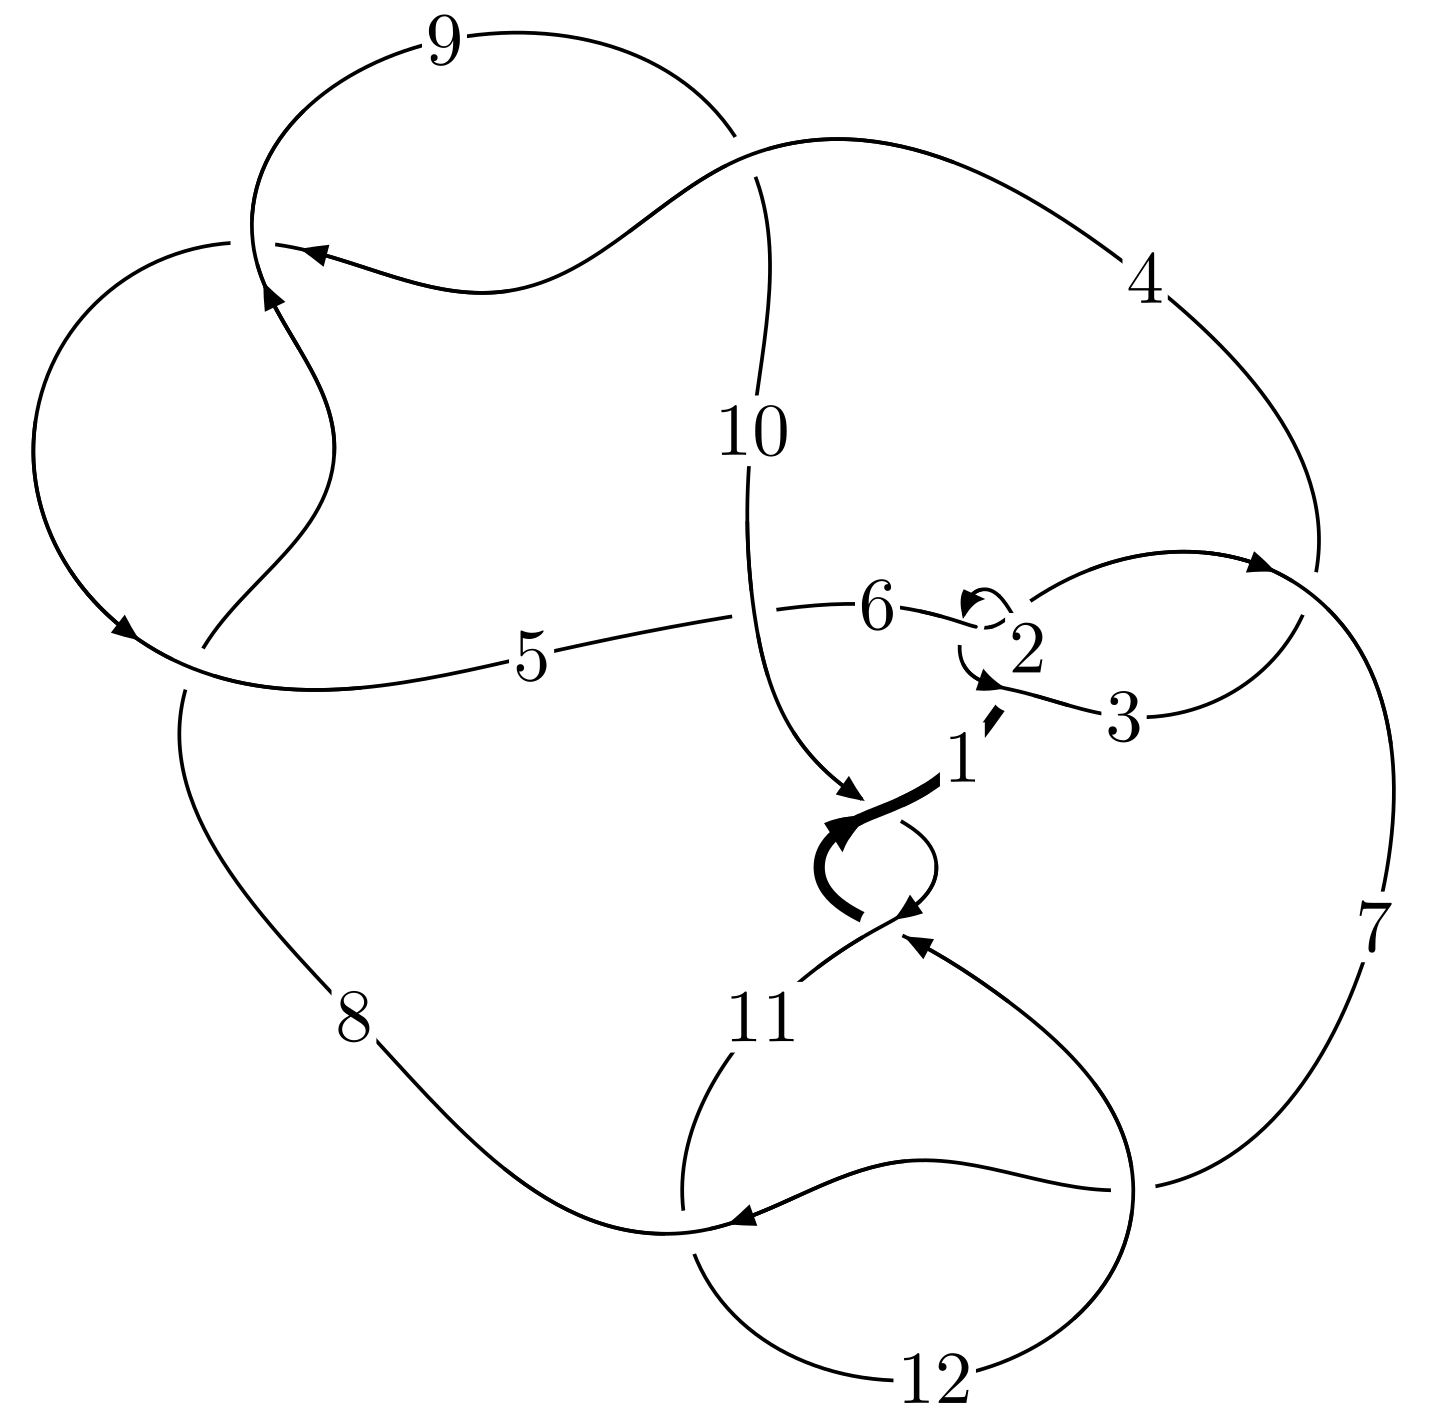
\includegraphics[width=112pt]{../../../GIT/diagram.site/Diagrams/png/1019_12a_0218.png}\\
\ \ \ A knot diagram\footnotemark}&
\allowdisplaybreaks
\textbf{Linearized knot diagam} \\
\cline{2-2}
 &
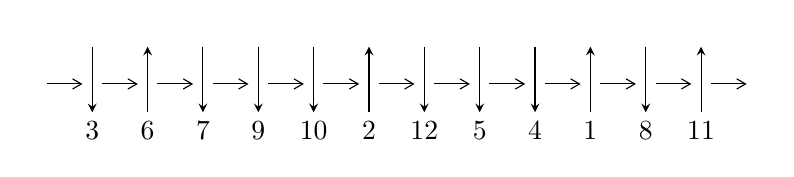
\begin{tikzpicture}[x=20pt, y=17pt]
	% nodes
	\node (C0) at (0, 0) {};
	\node (C1) at (1, 0) {};
	\node (C1U) at (1, +1) {};
	\node (C1D) at (1, -1) {3};

	\node (C2) at (2, 0) {};
	\node (C2U) at (2, +1) {};
	\node (C2D) at (2, -1) {6};

	\node (C3) at (3, 0) {};
	\node (C3U) at (3, +1) {};
	\node (C3D) at (3, -1) {7};

	\node (C4) at (4, 0) {};
	\node (C4U) at (4, +1) {};
	\node (C4D) at (4, -1) {9};

	\node (C5) at (5, 0) {};
	\node (C5U) at (5, +1) {};
	\node (C5D) at (5, -1) {10};

	\node (C6) at (6, 0) {};
	\node (C6U) at (6, +1) {};
	\node (C6D) at (6, -1) {2};

	\node (C7) at (7, 0) {};
	\node (C7U) at (7, +1) {};
	\node (C7D) at (7, -1) {12};

	\node (C8) at (8, 0) {};
	\node (C8U) at (8, +1) {};
	\node (C8D) at (8, -1) {5};

	\node (C9) at (9, 0) {};
	\node (C9U) at (9, +1) {};
	\node (C9D) at (9, -1) {4};

	\node (C10) at (10, 0) {};
	\node (C10U) at (10, +1) {};
	\node (C10D) at (10, -1) {1};

	\node (C11) at (11, 0) {};
	\node (C11U) at (11, +1) {};
	\node (C11D) at (11, -1) {8};

	\node (C12) at (12, 0) {};
	\node (C12U) at (12, +1) {};
	\node (C12D) at (12, -1) {11};
	\node (C13) at (13, 0) {};

	% arrows
	\draw[->,>={angle 60}]
	(C0) edge (C1) (C1) edge (C2) (C2) edge (C3) (C3) edge (C4) (C4) edge (C5) (C5) edge (C6) (C6) edge (C7) (C7) edge (C8) (C8) edge (C9) (C9) edge (C10) (C10) edge (C11) (C11) edge (C12) (C12) edge (C13) ;	\draw[->,>=stealth]
	(C1U) edge (C1D) (C2D) edge (C2U) (C3U) edge (C3D) (C4U) edge (C4D) (C5U) edge (C5D) (C6D) edge (C6U) (C7U) edge (C7D) (C8U) edge (C8D) (C9U) edge (C9D) (C10D) edge (C10U) (C11U) edge (C11D) (C12D) edge (C12U) ;
	\end{tikzpicture} \\
\hhline{~~} \\& 
\textbf{Solving Sequence} \\ \cline{2-2} 
 &
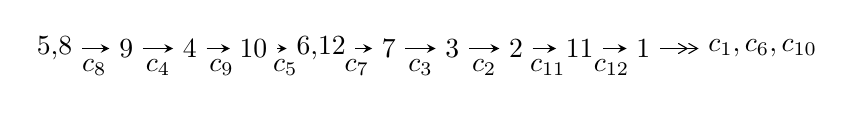
\begin{tikzpicture}[x=23pt, y=7pt]
	% node
	\node (A0) at (-1/8, 0) {5,8};
	\node (A1) at (1, 0) {9};
	\node (A2) at (2, 0) {4};
	\node (A3) at (3, 0) {10};
	\node (A4) at (65/16, 0) {6,12};
	\node (A5) at (41/8, 0) {7};
	\node (A6) at (49/8, 0) {3};
	\node (A7) at (57/8, 0) {2};
	\node (A8) at (65/8, 0) {11};
	\node (A9) at (73/8, 0) {1};
	\node (C1) at (1/2, -1) {$c_{8}$};
	\node (C2) at (3/2, -1) {$c_{4}$};
	\node (C3) at (5/2, -1) {$c_{9}$};
	\node (C4) at (7/2, -1) {$c_{5}$};
	\node (C5) at (37/8, -1) {$c_{7}$};
	\node (C6) at (45/8, -1) {$c_{3}$};
	\node (C7) at (53/8, -1) {$c_{2}$};
	\node (C8) at (61/8, -1) {$c_{11}$};
	\node (C9) at (69/8, -1) {$c_{12}$};
	\node (A10) at (11, 0) {$c_{1},c_{6},c_{10}$};

	% edge
	\draw[->,>=stealth]	
	(A0) edge (A1) (A1) edge (A2) (A2) edge (A3) (A3) edge (A4) (A4) edge (A5) (A5) edge (A6) (A6) edge (A7) (A7) edge (A8) (A8) edge (A9) ;
	\draw[->>,>={angle 60}]	
	(A9) edge (A10);
\end{tikzpicture} \\ 

\end{tabular} \\

\footnotetext{
The image of knot diagram is generated by the software ``\textbf{Draw programme}" developed by Andrew Bartholomew(\url{http://www.layer8.co.uk/maths/draw/index.htm\#Running-draw}), where we modified some parts for our purpose(\url{https://github.com/CATsTAILs/LinksPainter}).
}\phantom \\ \newline 
\centering \textbf{Ideals for irreducible components\footnotemark of $X_{\text{par}}$} 
 
\begin{align*}
I^u_{1}&=\langle 
1.83761\times10^{47} u^{83}+6.75612\times10^{47} u^{82}+\cdots+1.51134\times10^{48} b-6.34548\times10^{47},\\
\phantom{I^u_{1}}&\phantom{= \langle  }7.37805\times10^{46} u^{83}+2.42262\times10^{47} u^{82}+\cdots+7.55672\times10^{47} a+6.02649\times10^{48},\;u^{84}+4 u^{83}+\cdots+96 u+16\rangle \\
I^u_{2}&=\langle 
4 b+2 a- u+2,\;2 a^2-2 a u+5,\;u^2+2\rangle \\
I^u_{3}&=\langle 
-12751 a^4 u^2-3476 a^3 u^2+\cdots+134987 a-145138,\\
\phantom{I^u_{3}}&\phantom{= \langle  }2 a^4 u^2+a^5-2 a^3 u^2+2 a^4+3 a^3 u+4 a^2 u^2+a^3+2 a^2 u+5 u^2 a-4 a^2-2 a u-3 u^2+9 a+5 u-7,\\
\phantom{I^u_{3}}&\phantom{= \langle  }u^3- u^2+2 u-1\rangle \\
I^u_{4}&=\langle 
a u+9 b+4 a+u+4,\;2 a^2+a u-3 u+5,\;u^2+2\rangle \\
\\
I^v_{1}&=\langle 
a,\;b- v-1,\;v^2+v+1\rangle \\
I^v_{2}&=\langle 
a,\;b^2- b+1,\;v-1\rangle \\
\end{align*}
\raggedright * 6 irreducible components of $\dim_{\mathbb{C}}=0$, with total 111 representations.\\
\footnotetext{All coefficients of polynomials are rational numbers. But the coefficients are sometimes approximated in decimal forms when there is not enough margin.}
\newpage
\renewcommand{\arraystretch}{1}
\centering \section*{I. $I^u_{1}= \langle 1.84\times10^{47} u^{83}+6.76\times10^{47} u^{82}+\cdots+1.51\times10^{48} b-6.35\times10^{47},\;7.38\times10^{46} u^{83}+2.42\times10^{47} u^{82}+\cdots+7.56\times10^{47} a+6.03\times10^{48},\;u^{84}+4 u^{83}+\cdots+96 u+16 \rangle$}
\flushleft \textbf{(i) Arc colorings}\\
\begin{tabular}{m{7pt} m{180pt} m{7pt} m{180pt} }
\flushright $a_{5}=$&$\begin{pmatrix}0\\u\end{pmatrix}$ \\
\flushright $a_{8}=$&$\begin{pmatrix}1\\0\end{pmatrix}$ \\
\flushright $a_{9}=$&$\begin{pmatrix}1\\u^2\end{pmatrix}$ \\
\flushright $a_{4}=$&$\begin{pmatrix}u\\u^3+u\end{pmatrix}$ \\
\flushright $a_{10}=$&$\begin{pmatrix}u^2+1\\u^4+2 u^2\end{pmatrix}$ \\
\flushright $a_{6}=$&$\begin{pmatrix}- u^5-2 u^3- u\\- u^7-3 u^5-2 u^3+u\end{pmatrix}$ \\
\flushright $a_{12}=$&$\begin{pmatrix}-0.0976356 u^{83}-0.320592 u^{82}+\cdots-30.0041 u-7.97502\\-0.121588 u^{83}-0.447027 u^{82}+\cdots-3.28280 u+0.419857\end{pmatrix}$ \\
\flushright $a_{7}=$&$\begin{pmatrix}0.198396 u^{83}+0.413274 u^{82}+\cdots+2.76813 u+0.709068\\0.112403 u^{83}+0.314145 u^{82}+\cdots-2.45717 u-1.02935\end{pmatrix}$ \\
\flushright $a_{3}=$&$\begin{pmatrix}0.405056 u^{83}+1.56056 u^{82}+\cdots+59.3006 u+12.8650\\0.138509 u^{83}+0.543278 u^{82}+\cdots+26.3533 u+5.30097\end{pmatrix}$ \\
\flushright $a_{2}=$&$\begin{pmatrix}0.411073 u^{83}+1.58363 u^{82}+\cdots+39.6138 u+7.75297\\0.123419 u^{83}+0.481396 u^{82}+\cdots+31.0917 u+6.38943\end{pmatrix}$ \\
\flushright $a_{11}=$&$\begin{pmatrix}-0.219223 u^{83}-0.767619 u^{82}+\cdots-33.2869 u-7.55516\\-0.121588 u^{83}-0.447027 u^{82}+\cdots-3.28280 u+0.419857\end{pmatrix}$ \\
\flushright $a_{1}=$&$\begin{pmatrix}0.325649 u^{83}+1.35250 u^{82}+\cdots+47.3100 u+8.96150\\0.0405219 u^{83}+0.178471 u^{82}+\cdots+36.9975 u+8.48326\end{pmatrix}$\\&\end{tabular}
\flushleft \textbf{(ii) Obstruction class $= -1$}\\~\\
\flushleft \textbf{(iii) Cusp Shapes $= -1.25888 u^{83}-3.47330 u^{82}+\cdots-45.0684 u-15.7517$}\\~\\
\newpage\renewcommand{\arraystretch}{1}
\flushleft \textbf{(iv) u-Polynomials at the component}\newline \\
\begin{tabular}{m{50pt}|m{274pt}}
Crossings & \hspace{64pt}u-Polynomials at each crossing \\
\hline $$\begin{aligned}c_{1}\end{aligned}$$&$\begin{aligned}
&u^{84}+43 u^{83}+\cdots+80 u+9
\end{aligned}$\\
\hline $$\begin{aligned}c_{2},c_{6}\end{aligned}$$&$\begin{aligned}
&u^{84}-3 u^{83}+\cdots-8 u+3
\end{aligned}$\\
\hline $$\begin{aligned}c_{3}\end{aligned}$$&$\begin{aligned}
&u^{84}+3 u^{83}+\cdots+44270 u+12039
\end{aligned}$\\
\hline $$\begin{aligned}c_{4},c_{8},c_{9}\end{aligned}$$&$\begin{aligned}
&u^{84}-4 u^{83}+\cdots-96 u+16
\end{aligned}$\\
\hline $$\begin{aligned}c_{5}\end{aligned}$$&$\begin{aligned}
&u^{84}+4 u^{83}+\cdots+192992 u+185296
\end{aligned}$\\
\hline $$\begin{aligned}c_{7},c_{11}\end{aligned}$$&$\begin{aligned}
&u^{84}+3 u^{83}+\cdots-22 u+3
\end{aligned}$\\
\hline $$\begin{aligned}c_{10},c_{12}\end{aligned}$$&$\begin{aligned}
&u^{84}-27 u^{83}+\cdots-80 u+9
\end{aligned}$\\
\hline
\end{tabular}\\~\\
\newpage\renewcommand{\arraystretch}{1}
\flushleft \textbf{(v) Riley Polynomials at the component}\newline \\
\begin{tabular}{m{50pt}|m{274pt}}
Crossings & \hspace{64pt}Riley Polynomials at each crossing \\
\hline $$\begin{aligned}c_{1}\end{aligned}$$&$\begin{aligned}
&y^{84}+3 y^{83}+\cdots+1988 y+81
\end{aligned}$\\
\hline $$\begin{aligned}c_{2},c_{6}\end{aligned}$$&$\begin{aligned}
&y^{84}+43 y^{83}+\cdots+80 y+9
\end{aligned}$\\
\hline $$\begin{aligned}c_{3}\end{aligned}$$&$\begin{aligned}
&y^{84}-37 y^{83}+\cdots+1982120948 y+144937521
\end{aligned}$\\
\hline $$\begin{aligned}c_{4},c_{8},c_{9}\end{aligned}$$&$\begin{aligned}
&y^{84}+76 y^{83}+\cdots+9728 y^2+256
\end{aligned}$\\
\hline $$\begin{aligned}c_{5}\end{aligned}$$&$\begin{aligned}
&y^{84}-4 y^{83}+\cdots+562686205952 y+34334607616
\end{aligned}$\\
\hline $$\begin{aligned}c_{7},c_{11}\end{aligned}$$&$\begin{aligned}
&y^{84}+27 y^{83}+\cdots+80 y+9
\end{aligned}$\\
\hline $$\begin{aligned}c_{10},c_{12}\end{aligned}$$&$\begin{aligned}
&y^{84}+67 y^{83}+\cdots+35684 y+81
\end{aligned}$\\
\hline
\end{tabular}\\~\\
\newpage\flushleft \textbf{(vi) Complex Volumes and Cusp Shapes}
$$\begin{array}{c|c|c}  
\text{Solutions to }I^u_{1}& \I (\text{vol} + \sqrt{-1}CS) & \text{Cusp shape}\\
 \hline 
\begin{aligned}
u &= \phantom{-}0.350754 + 0.942596 I \\
a &= \phantom{-}0.642858 - 0.879615 I \\
b &= \phantom{-}0.771585 + 0.815019 I\end{aligned}
 & -2.14146 - 2.52752 I & \phantom{-0.000000 } 0 \\ \hline\begin{aligned}
u &= \phantom{-}0.350754 - 0.942596 I \\
a &= \phantom{-}0.642858 + 0.879615 I \\
b &= \phantom{-}0.771585 - 0.815019 I\end{aligned}
 & -2.14146 + 2.52752 I & \phantom{-0.000000 } 0 \\ \hline\begin{aligned}
u &= \phantom{-}0.540304 + 0.822649 I \\
a &= -0.042257 + 0.688019 I \\
b &= \phantom{-}0.755822 - 0.974029 I\end{aligned}
 & -4.62886 + 7.84102 I & \phantom{-0.000000 } 0 \\ \hline\begin{aligned}
u &= \phantom{-}0.540304 - 0.822649 I \\
a &= -0.042257 - 0.688019 I \\
b &= \phantom{-}0.755822 + 0.974029 I\end{aligned}
 & -4.62886 - 7.84102 I & \phantom{-0.000000 } 0 \\ \hline\begin{aligned}
u &= -0.495294 + 0.887879 I \\
a &= \phantom{-}0.473834 + 0.922359 I \\
b &= \phantom{-}0.821705 - 0.771878 I\end{aligned}
 & -5.25459 - 1.93039 I & \phantom{-0.000000 } 0 \\ \hline\begin{aligned}
u &= -0.495294 - 0.887879 I \\
a &= \phantom{-}0.473834 - 0.922359 I \\
b &= \phantom{-}0.821705 + 0.771878 I\end{aligned}
 & -5.25459 + 1.93039 I & \phantom{-0.000000 } 0 \\ \hline\begin{aligned}
u &= -0.408826 + 0.824363 I \\
a &= \phantom{-}0.073344 - 0.595451 I \\
b &= \phantom{-}0.731673 + 0.929862 I\end{aligned}
 & -1.78240 - 3.16007 I & \phantom{-0.000000 } 0 \\ \hline\begin{aligned}
u &= -0.408826 - 0.824363 I \\
a &= \phantom{-}0.073344 + 0.595451 I \\
b &= \phantom{-}0.731673 - 0.929862 I\end{aligned}
 & -1.78240 + 3.16007 I & \phantom{-0.000000 } 0 \\ \hline\begin{aligned}
u &= \phantom{-}0.449775 + 0.998287 I \\
a &= -0.107414 + 0.446418 I \\
b &= \phantom{-}0.793035 - 0.902515 I\end{aligned}
 & -5.77493 - 0.50478 I & \phantom{-0.000000 } 0 \\ \hline\begin{aligned}
u &= \phantom{-}0.449775 - 0.998287 I \\
a &= -0.107414 - 0.446418 I \\
b &= \phantom{-}0.793035 + 0.902515 I\end{aligned}
 & -5.77493 + 0.50478 I & \phantom{-0.000000 } 0\\
 \hline 
 \end{array}$$\newpage$$\begin{array}{c|c|c}  
\text{Solutions to }I^u_{1}& \I (\text{vol} + \sqrt{-1}CS) & \text{Cusp shape}\\
 \hline 
\begin{aligned}
u &= \phantom{-}0.826469 + 0.301584 I \\
a &= -1.43413 + 1.02708 I \\
b &= -0.752423 - 1.020840 I\end{aligned}
 & -6.29688 - 12.60120 I & -7.95324 + 9.37514 I \\ \hline\begin{aligned}
u &= \phantom{-}0.826469 - 0.301584 I \\
a &= -1.43413 - 1.02708 I \\
b &= -0.752423 + 1.020840 I\end{aligned}
 & -6.29688 + 12.60120 I & -7.95324 - 9.37514 I \\ \hline\begin{aligned}
u &= -0.829199 + 0.256834 I \\
a &= -0.196573 - 0.451034 I \\
b &= -0.858127 - 0.711648 I\end{aligned}
 & -7.24866 + 6.60173 I & -9.74629 - 4.48762 I \\ \hline\begin{aligned}
u &= -0.829199 - 0.256834 I \\
a &= -0.196573 + 0.451034 I \\
b &= -0.858127 + 0.711648 I\end{aligned}
 & -7.24866 - 6.60173 I & -9.74629 + 4.48762 I \\ \hline\begin{aligned}
u &= \phantom{-}0.834377 + 0.184117 I \\
a &= -1.35063 + 0.57913 I \\
b &= -0.779630 - 0.965446 I\end{aligned}
 & -8.29808 - 4.07556 I & -10.87765 + 3.19682 I \\ \hline\begin{aligned}
u &= \phantom{-}0.834377 - 0.184117 I \\
a &= -1.35063 - 0.57913 I \\
b &= -0.779630 + 0.965446 I\end{aligned}
 & -8.29808 + 4.07556 I & -10.87765 - 3.19682 I \\ \hline\begin{aligned}
u &= -0.839410 + 0.127426 I \\
a &= -0.581311 - 0.311001 I \\
b &= -0.839261 - 0.795078 I\end{aligned}
 & -8.82615 - 1.96225 I & -11.76893 + 2.26917 I \\ \hline\begin{aligned}
u &= -0.839410 - 0.127426 I \\
a &= -0.581311 + 0.311001 I \\
b &= -0.839261 + 0.795078 I\end{aligned}
 & -8.82615 + 1.96225 I & -11.76893 - 2.26917 I \\ \hline\begin{aligned}
u &= -0.433217 + 1.076530 I \\
a &= \phantom{-}0.663567 + 1.117850 I \\
b &= \phantom{-}0.814296 - 0.862710 I\end{aligned}
 & -5.90386 + 6.51028 I & \phantom{-0.000000 } 0 \\ \hline\begin{aligned}
u &= -0.433217 - 1.076530 I \\
a &= \phantom{-}0.663567 - 1.117850 I \\
b &= \phantom{-}0.814296 + 0.862710 I\end{aligned}
 & -5.90386 - 6.51028 I & \phantom{-0.000000 } 0\\
 \hline 
 \end{array}$$\newpage$$\begin{array}{c|c|c}  
\text{Solutions to }I^u_{1}& \I (\text{vol} + \sqrt{-1}CS) & \text{Cusp shape}\\
 \hline 
\begin{aligned}
u &= -0.783250 + 0.264115 I \\
a &= -1.60999 - 0.87791 I \\
b &= -0.739512 + 0.994581 I\end{aligned}
 & -3.62130 + 7.46949 I & -5.36276 - 6.04622 I \\ \hline\begin{aligned}
u &= -0.783250 - 0.264115 I \\
a &= -1.60999 + 0.87791 I \\
b &= -0.739512 - 0.994581 I\end{aligned}
 & -3.62130 - 7.46949 I & -5.36276 + 6.04622 I \\ \hline\begin{aligned}
u &= \phantom{-}0.068050 + 1.173920 I \\
a &= \phantom{-}0.11077 - 2.34272 I \\
b &= -0.412731 + 1.054140 I\end{aligned}
 & \phantom{-}2.11004 + 4.12289 I & \phantom{-0.000000 } 0 \\ \hline\begin{aligned}
u &= \phantom{-}0.068050 - 1.173920 I \\
a &= \phantom{-}0.11077 + 2.34272 I \\
b &= -0.412731 - 1.054140 I\end{aligned}
 & \phantom{-}2.11004 - 4.12289 I & \phantom{-0.000000 } 0 \\ \hline\begin{aligned}
u &= -0.239259 + 1.168840 I \\
a &= \phantom{-}0.380988 - 0.383419 I \\
b &= -0.714493 + 0.091333 I\end{aligned}
 & -0.762339 - 0.275947 I & \phantom{-0.000000 } 0 \\ \hline\begin{aligned}
u &= -0.239259 - 1.168840 I \\
a &= \phantom{-}0.380988 + 0.383419 I \\
b &= -0.714493 - 0.091333 I\end{aligned}
 & -0.762339 + 0.275947 I & \phantom{-0.000000 } 0 \\ \hline\begin{aligned}
u &= \phantom{-}0.777544 + 0.209804 I \\
a &= -0.362630 + 0.599070 I \\
b &= -0.815410 + 0.732335 I\end{aligned}
 & -4.42446 - 1.63033 I & -7.06387 + 0.91981 I \\ \hline\begin{aligned}
u &= \phantom{-}0.777544 - 0.209804 I \\
a &= -0.362630 - 0.599070 I \\
b &= -0.815410 - 0.732335 I\end{aligned}
 & -4.42446 + 1.63033 I & -7.06387 - 0.91981 I \\ \hline\begin{aligned}
u &= -0.168003 + 1.255030 I \\
a &= -0.019540 + 0.607170 I \\
b &= \phantom{-}0.711034 + 0.763554 I\end{aligned}
 & \phantom{-}2.47373 - 2.56298 I & \phantom{-0.000000 } 0 \\ \hline\begin{aligned}
u &= -0.168003 - 1.255030 I \\
a &= -0.019540 - 0.607170 I \\
b &= \phantom{-}0.711034 - 0.763554 I\end{aligned}
 & \phantom{-}2.47373 + 2.56298 I & \phantom{-0.000000 } 0\\
 \hline 
 \end{array}$$\newpage$$\begin{array}{c|c|c}  
\text{Solutions to }I^u_{1}& \I (\text{vol} + \sqrt{-1}CS) & \text{Cusp shape}\\
 \hline 
\begin{aligned}
u &= -0.713006 + 0.095615 I \\
a &= \phantom{-}0.334802 + 0.120967 I \\
b &= \phantom{-}0.722210 - 0.106046 I\end{aligned}
 & -3.96162 + 3.79092 I & -11.61122 - 4.56726 I \\ \hline\begin{aligned}
u &= -0.713006 - 0.095615 I \\
a &= \phantom{-}0.334802 - 0.120967 I \\
b &= \phantom{-}0.722210 + 0.106046 I\end{aligned}
 & -3.96162 - 3.79092 I & -11.61122 + 4.56726 I \\ \hline\begin{aligned}
u &= \phantom{-}0.668399 + 0.237900 I \\
a &= \phantom{-}0.67448 - 1.39382 I \\
b &= \phantom{-}0.213868 + 1.083920 I\end{aligned}
 & -0.04595 - 6.79511 I & -4.41057 + 8.39005 I \\ \hline\begin{aligned}
u &= \phantom{-}0.668399 - 0.237900 I \\
a &= \phantom{-}0.67448 + 1.39382 I \\
b &= \phantom{-}0.213868 - 1.083920 I\end{aligned}
 & -0.04595 + 6.79511 I & -4.41057 - 8.39005 I \\ \hline\begin{aligned}
u &= -0.288293 + 1.320130 I \\
a &= \phantom{-}0.367736 - 0.623675 I \\
b &= -0.776388 + 0.237242 I\end{aligned}
 & \phantom{-}0.47634 + 7.41480 I & \phantom{-0.000000 } 0 \\ \hline\begin{aligned}
u &= -0.288293 - 1.320130 I \\
a &= \phantom{-}0.367736 + 0.623675 I \\
b &= -0.776388 - 0.237242 I\end{aligned}
 & \phantom{-}0.47634 - 7.41480 I & \phantom{-0.000000 } 0 \\ \hline\begin{aligned}
u &= -0.576067 + 0.282806 I \\
a &= \phantom{-}0.82703 + 1.32861 I \\
b &= \phantom{-}0.165831 - 1.001990 I\end{aligned}
 & \phantom{-}2.06976 + 2.29339 I & -0.00881 - 4.82687 I \\ \hline\begin{aligned}
u &= -0.576067 - 0.282806 I \\
a &= \phantom{-}0.82703 - 1.32861 I \\
b &= \phantom{-}0.165831 + 1.001990 I\end{aligned}
 & \phantom{-}2.06976 - 2.29339 I & -0.00881 + 4.82687 I \\ \hline\begin{aligned}
u &= -0.132078 + 1.355200 I \\
a &= \phantom{-}0.22554 + 2.00262 I \\
b &= -0.514621 - 1.021830 I\end{aligned}
 & \phantom{-}5.19651 - 1.43194 I & \phantom{-0.000000 } 0 \\ \hline\begin{aligned}
u &= -0.132078 - 1.355200 I \\
a &= \phantom{-}0.22554 - 2.00262 I \\
b &= -0.514621 + 1.021830 I\end{aligned}
 & \phantom{-}5.19651 + 1.43194 I & \phantom{-0.000000 } 0\\
 \hline 
 \end{array}$$\newpage$$\begin{array}{c|c|c}  
\text{Solutions to }I^u_{1}& \I (\text{vol} + \sqrt{-1}CS) & \text{Cusp shape}\\
 \hline 
\begin{aligned}
u &= -0.247258 + 1.348180 I \\
a &= \phantom{-}1.55578 + 1.82417 I \\
b &= \phantom{-}0.698833 - 0.975302 I\end{aligned}
 & \phantom{-}3.79061 + 8.31615 I & \phantom{-0.000000 } 0 \\ \hline\begin{aligned}
u &= -0.247258 - 1.348180 I \\
a &= \phantom{-}1.55578 - 1.82417 I \\
b &= \phantom{-}0.698833 + 0.975302 I\end{aligned}
 & \phantom{-}3.79061 - 8.31615 I & \phantom{-0.000000 } 0 \\ \hline\begin{aligned}
u &= -0.362756 + 1.332060 I \\
a &= -0.581243 + 0.024357 I \\
b &= \phantom{-}0.851771 + 0.728928 I\end{aligned}
 & -4.25572 + 2.35314 I & \phantom{-0.000000 } 0 \\ \hline\begin{aligned}
u &= -0.362756 - 1.332060 I \\
a &= -0.581243 - 0.024357 I \\
b &= \phantom{-}0.851771 - 0.728928 I\end{aligned}
 & -4.25572 - 2.35314 I & \phantom{-0.000000 } 0 \\ \hline\begin{aligned}
u &= \phantom{-}0.038709 + 1.381560 I \\
a &= -0.681056 + 0.333747 I \\
b &= -0.200806 - 0.178820 I\end{aligned}
 & \phantom{-}4.96495 - 2.19922 I & \phantom{-0.000000 } 0 \\ \hline\begin{aligned}
u &= \phantom{-}0.038709 - 1.381560 I \\
a &= -0.681056 - 0.333747 I \\
b &= -0.200806 + 0.178820 I\end{aligned}
 & \phantom{-}4.96495 + 2.19922 I & \phantom{-0.000000 } 0 \\ \hline\begin{aligned}
u &= -0.600064 + 0.128543 I \\
a &= -2.60142 + 0.17153 I \\
b &= -0.673393 + 0.902935 I\end{aligned}
 & -0.89912 + 5.19420 I & -7.11874 - 7.76852 I \\ \hline\begin{aligned}
u &= -0.600064 - 0.128543 I \\
a &= -2.60142 - 0.17153 I \\
b &= -0.673393 - 0.902935 I\end{aligned}
 & -0.89912 - 5.19420 I & -7.11874 + 7.76852 I \\ \hline\begin{aligned}
u &= -0.454019 + 0.410951 I \\
a &= \phantom{-}1.32194 + 1.40913 I \\
b &= -0.032813 - 0.909390 I\end{aligned}
 & \phantom{-}2.60505 + 0.90512 I & \phantom{-}2.28754 - 4.05492 I \\ \hline\begin{aligned}
u &= -0.454019 - 0.410951 I \\
a &= \phantom{-}1.32194 - 1.40913 I \\
b &= -0.032813 + 0.909390 I\end{aligned}
 & \phantom{-}2.60505 - 0.90512 I & \phantom{-}2.28754 + 4.05492 I\\
 \hline 
 \end{array}$$\newpage$$\begin{array}{c|c|c}  
\text{Solutions to }I^u_{1}& \I (\text{vol} + \sqrt{-1}CS) & \text{Cusp shape}\\
 \hline 
\begin{aligned}
u &= -0.23621 + 1.39451 I \\
a &= -0.71816 - 2.47299 I \\
b &= -0.144636 + 1.099660 I\end{aligned}
 & \phantom{-}7.38356 + 5.30799 I & \phantom{-0.000000 } 0 \\ \hline\begin{aligned}
u &= -0.23621 - 1.39451 I \\
a &= -0.71816 + 2.47299 I \\
b &= -0.144636 - 1.099660 I\end{aligned}
 & \phantom{-}7.38356 - 5.30799 I & \phantom{-0.000000 } 0 \\ \hline\begin{aligned}
u &= \phantom{-}0.35405 + 1.37132 I \\
a &= \phantom{-}1.00055 - 1.87993 I \\
b &= \phantom{-}0.757561 + 1.008790 I\end{aligned}
 & -3.39478 - 8.35215 I & \phantom{-0.000000 } 0 \\ \hline\begin{aligned}
u &= \phantom{-}0.35405 - 1.37132 I \\
a &= \phantom{-}1.00055 + 1.87993 I \\
b &= \phantom{-}0.757561 - 1.008790 I\end{aligned}
 & -3.39478 + 8.35215 I & \phantom{-0.000000 } 0 \\ \hline\begin{aligned}
u &= \phantom{-}0.27368 + 1.39259 I \\
a &= -0.67813 + 2.52469 I \\
b &= -0.157124 - 1.142510 I\end{aligned}
 & \phantom{-}5.14150 - 10.24960 I & \phantom{-0.000000 } 0 \\ \hline\begin{aligned}
u &= \phantom{-}0.27368 - 1.39259 I \\
a &= -0.67813 - 2.52469 I \\
b &= -0.157124 + 1.142510 I\end{aligned}
 & \phantom{-}5.14150 + 10.24960 I & \phantom{-0.000000 } 0 \\ \hline\begin{aligned}
u &= \phantom{-}0.354969 + 0.458153 I \\
a &= \phantom{-}1.89488 - 1.64861 I \\
b &= -0.181249 + 0.882030 I\end{aligned}
 & \phantom{-}1.20125 + 3.56606 I & \phantom{-}0.00892 - 1.69990 I \\ \hline\begin{aligned}
u &= \phantom{-}0.354969 - 0.458153 I \\
a &= \phantom{-}1.89488 + 1.64861 I \\
b &= -0.181249 - 0.882030 I\end{aligned}
 & \phantom{-}1.20125 - 3.56606 I & \phantom{-}0.00892 + 1.69990 I \\ \hline\begin{aligned}
u &= \phantom{-}0.31969 + 1.38632 I \\
a &= -0.720461 - 0.134519 I \\
b &= \phantom{-}0.839786 - 0.673215 I\end{aligned}
 & \phantom{-}0.63547 - 5.59776 I & \phantom{-0.000000 } 0 \\ \hline\begin{aligned}
u &= \phantom{-}0.31969 - 1.38632 I \\
a &= -0.720461 + 0.134519 I \\
b &= \phantom{-}0.839786 + 0.673215 I\end{aligned}
 & \phantom{-}0.63547 + 5.59776 I & \phantom{-0.000000 } 0\\
 \hline 
 \end{array}$$\newpage$$\begin{array}{c|c|c}  
\text{Solutions to }I^u_{1}& \I (\text{vol} + \sqrt{-1}CS) & \text{Cusp shape}\\
 \hline 
\begin{aligned}
u &= -0.16228 + 1.42710 I \\
a &= -0.95852 - 2.33237 I \\
b &= -0.069061 + 0.988963 I\end{aligned}
 & \phantom{-}8.46071 + 3.17427 I & \phantom{-0.000000 } 0 \\ \hline\begin{aligned}
u &= -0.16228 - 1.42710 I \\
a &= -0.95852 + 2.33237 I \\
b &= -0.069061 - 0.988963 I\end{aligned}
 & \phantom{-}8.46071 - 3.17427 I & \phantom{-0.000000 } 0 \\ \hline\begin{aligned}
u &= \phantom{-}0.07272 + 1.44133 I \\
a &= -0.081833 + 1.365030 I \\
b &= -0.512649 - 0.683277 I\end{aligned}
 & \phantom{-}4.65094 - 2.50593 I & \phantom{-0.000000 } 0 \\ \hline\begin{aligned}
u &= \phantom{-}0.07272 - 1.44133 I \\
a &= -0.081833 - 1.365030 I \\
b &= -0.512649 + 0.683277 I\end{aligned}
 & \phantom{-}4.65094 + 2.50593 I & \phantom{-0.000000 } 0 \\ \hline\begin{aligned}
u &= \phantom{-}0.13184 + 1.43845 I \\
a &= -1.17422 + 2.21897 I \\
b &= -0.018498 - 0.919588 I\end{aligned}
 & \phantom{-}7.23839 + 1.71145 I & \phantom{-0.000000 } 0 \\ \hline\begin{aligned}
u &= \phantom{-}0.13184 - 1.43845 I \\
a &= -1.17422 - 2.21897 I \\
b &= -0.018498 + 0.919588 I\end{aligned}
 & \phantom{-}7.23839 - 1.71145 I & \phantom{-0.000000 } 0 \\ \hline\begin{aligned}
u &= -0.31835 + 1.41515 I \\
a &= \phantom{-}1.08570 + 2.10712 I \\
b &= \phantom{-}0.728768 - 1.031050 I\end{aligned}
 & \phantom{-}1.72641 + 11.46270 I & \phantom{-0.000000 } 0 \\ \hline\begin{aligned}
u &= -0.31835 - 1.41515 I \\
a &= \phantom{-}1.08570 - 2.10712 I \\
b &= \phantom{-}0.728768 + 1.031050 I\end{aligned}
 & \phantom{-}1.72641 - 11.46270 I & \phantom{-0.000000 } 0 \\ \hline\begin{aligned}
u &= -0.34234 + 1.41472 I \\
a &= -0.781229 + 0.066281 I \\
b &= \phantom{-}0.870421 + 0.660227 I\end{aligned}
 & -1.93901 + 10.83450 I & \phantom{-0.000000 } 0 \\ \hline\begin{aligned}
u &= -0.34234 - 1.41472 I \\
a &= -0.781229 - 0.066281 I \\
b &= \phantom{-}0.870421 - 0.660227 I\end{aligned}
 & -1.93901 - 10.83450 I & \phantom{-0.000000 } 0\\
 \hline 
 \end{array}$$\newpage$$\begin{array}{c|c|c}  
\text{Solutions to }I^u_{1}& \I (\text{vol} + \sqrt{-1}CS) & \text{Cusp shape}\\
 \hline 
\begin{aligned}
u &= -0.07678 + 1.47131 I \\
a &= \phantom{-}0.25274 + 1.75932 I \\
b &= -0.604385 - 0.938277 I\end{aligned}
 & \phantom{-}5.41135 - 2.06230 I & \phantom{-0.000000 } 0 \\ \hline\begin{aligned}
u &= -0.07678 - 1.47131 I \\
a &= \phantom{-}0.25274 - 1.75932 I \\
b &= -0.604385 + 0.938277 I\end{aligned}
 & \phantom{-}5.41135 + 2.06230 I & \phantom{-0.000000 } 0 \\ \hline\begin{aligned}
u &= \phantom{-}0.33452 + 1.43819 I \\
a &= \phantom{-}0.97375 - 2.16552 I \\
b &= \phantom{-}0.735962 + 1.048690 I\end{aligned}
 & -0.7474 - 16.8065 I & \phantom{-0.000000 } 0 \\ \hline\begin{aligned}
u &= \phantom{-}0.33452 - 1.43819 I \\
a &= \phantom{-}0.97375 + 2.16552 I \\
b &= \phantom{-}0.735962 - 1.048690 I\end{aligned}
 & -0.7474 + 16.8065 I & \phantom{-0.000000 } 0 \\ \hline\begin{aligned}
u &= \phantom{-}0.409816 + 0.325133 I \\
a &= \phantom{-}0.638033 - 0.588897 I \\
b &= \phantom{-}0.475752 + 0.559238 I\end{aligned}
 & -1.05079 - 0.99662 I & -8.88984 + 5.17874 I \\ \hline\begin{aligned}
u &= \phantom{-}0.409816 - 0.325133 I \\
a &= \phantom{-}0.638033 + 0.588897 I \\
b &= \phantom{-}0.475752 - 0.559238 I\end{aligned}
 & -1.05079 + 0.99662 I & -8.88984 - 5.17874 I \\ \hline\begin{aligned}
u &= \phantom{-}0.226772 + 0.416872 I \\
a &= \phantom{-}1.164160 + 0.133562 I \\
b &= -0.317397 + 0.274980 I\end{aligned}
 & -0.50948 - 1.44830 I & -5.05239 + 5.14744 I \\ \hline\begin{aligned}
u &= \phantom{-}0.226772 - 0.416872 I \\
a &= \phantom{-}1.164160 - 0.133562 I \\
b &= -0.317397 - 0.274980 I\end{aligned}
 & -0.50948 + 1.44830 I & -5.05239 - 5.14744 I \\ \hline\begin{aligned}
u &= -0.02923 + 1.54028 I \\
a &= \phantom{-}0.29040 - 1.47834 I \\
b &= -0.696662 + 0.798330 I\end{aligned}
 & \phantom{-}2.96237 - 0.76259 I & \phantom{-0.000000 } 0 \\ \hline\begin{aligned}
u &= -0.02923 - 1.54028 I \\
a &= \phantom{-}0.29040 + 1.47834 I \\
b &= -0.696662 - 0.798330 I\end{aligned}
 & \phantom{-}2.96237 + 0.76259 I & \phantom{-0.000000 } 0\\
 \hline 
 \end{array}$$\newpage$$\begin{array}{c|c|c}  
\text{Solutions to }I^u_{1}& \I (\text{vol} + \sqrt{-1}CS) & \text{Cusp shape}\\
 \hline 
\begin{aligned}
u &= -0.367236 + 0.275592 I \\
a &= \phantom{-}0.364861 - 0.926737 I \\
b &= \phantom{-}0.540306 + 0.956806 I\end{aligned}
 & \phantom{-}0.03876 - 3.21058 I & -4.83770 - 1.13154 I \\ \hline\begin{aligned}
u &= -0.367236 - 0.275592 I \\
a &= \phantom{-}0.364861 + 0.926737 I \\
b &= \phantom{-}0.540306 - 0.956806 I\end{aligned}
 & \phantom{-}0.03876 + 3.21058 I & -4.83770 + 1.13154 I \\ \hline\begin{aligned}
u &= \phantom{-}0.06999 + 1.54596 I \\
a &= \phantom{-}0.36301 - 1.66914 I \\
b &= -0.688951 + 0.926678 I\end{aligned}
 & \phantom{-}3.36051 + 6.09970 I & \phantom{-0.000000 } 0 \\ \hline\begin{aligned}
u &= \phantom{-}0.06999 - 1.54596 I \\
a &= \phantom{-}0.36301 + 1.66914 I \\
b &= -0.688951 - 0.926678 I\end{aligned}
 & \phantom{-}3.36051 - 6.09970 I & \phantom{-0.000000 } 0\\
 \hline 
 \end{array}$$\newpage\newpage\renewcommand{\arraystretch}{1}
\centering \section*{II. $I^u_{2}= \langle 4 b+2 a- u+2,\;2 a^2-2 a u+5,\;u^2+2 \rangle$}
\flushleft \textbf{(i) Arc colorings}\\
\begin{tabular}{m{7pt} m{180pt} m{7pt} m{180pt} }
\flushright $a_{5}=$&$\begin{pmatrix}0\\u\end{pmatrix}$ \\
\flushright $a_{8}=$&$\begin{pmatrix}1\\0\end{pmatrix}$ \\
\flushright $a_{9}=$&$\begin{pmatrix}1\\-2\end{pmatrix}$ \\
\flushright $a_{4}=$&$\begin{pmatrix}u\\- u\end{pmatrix}$ \\
\flushright $a_{10}=$&$\begin{pmatrix}-1\\0\end{pmatrix}$ \\
\flushright $a_{6}=$&$\begin{pmatrix}- u\\u\end{pmatrix}$ \\
\flushright $a_{12}=$&$\begin{pmatrix}a\\-\frac{1}{2} a+\frac{1}{4} u-\frac{1}{2}\end{pmatrix}$ \\
\flushright $a_{7}=$&$\begin{pmatrix}\frac{1}{4} a u+\frac{1}{2} a-\frac{1}{4}\\-\frac{1}{2} a+\frac{1}{4} u+\frac{1}{2}\end{pmatrix}$ \\
\flushright $a_{3}=$&$\begin{pmatrix}\frac{1}{4} a u+\frac{3}{4} u-\frac{3}{4}\\- u+1\end{pmatrix}$ \\
\flushright $a_{2}=$&$\begin{pmatrix}\frac{3}{4} a u+\frac{1}{4} u-\frac{1}{4}\\-\frac{1}{2} a u-\frac{1}{2} u+\frac{1}{2}\end{pmatrix}$ \\
\flushright $a_{11}=$&$\begin{pmatrix}\frac{1}{2} a+\frac{1}{4} u-\frac{1}{2}\\-\frac{1}{2} a+\frac{1}{4} u-\frac{1}{2}\end{pmatrix}$ \\
\flushright $a_{1}=$&$\begin{pmatrix}\frac{1}{4} a u+\frac{1}{2} a-\frac{1}{4}\\-\frac{1}{2} a+\frac{1}{4} u+\frac{1}{2}\end{pmatrix}$\\&\end{tabular}
\flushleft \textbf{(ii) Obstruction class $= 1$}\\~\\
\flushleft \textbf{(iii) Cusp Shapes $= 4 a-2 u$}\\~\\
\newpage\renewcommand{\arraystretch}{1}
\flushleft \textbf{(iv) u-Polynomials at the component}\newline \\
\begin{tabular}{m{50pt}|m{274pt}}
Crossings & \hspace{64pt}u-Polynomials at each crossing \\
\hline $$\begin{aligned}c_{1},c_{2},c_{11}\\c_{12}\end{aligned}$$&$\begin{aligned}
&(u^2- u+1)^2
\end{aligned}$\\
\hline $$\begin{aligned}c_{3},c_{6},c_{7}\\c_{10}\end{aligned}$$&$\begin{aligned}
&(u^2+u+1)^2
\end{aligned}$\\
\hline $$\begin{aligned}c_{4},c_{5},c_{8}\\c_{9}\end{aligned}$$&$\begin{aligned}
&(u^2+2)^2
\end{aligned}$\\
\hline
\end{tabular}\\~\\
\newpage\renewcommand{\arraystretch}{1}
\flushleft \textbf{(v) Riley Polynomials at the component}\newline \\
\begin{tabular}{m{50pt}|m{274pt}}
Crossings & \hspace{64pt}Riley Polynomials at each crossing \\
\hline $$\begin{aligned}c_{1},c_{2},c_{3}\\c_{6},c_{7},c_{10}\\c_{11},c_{12}\end{aligned}$$&$\begin{aligned}
&(y^2+y+1)^2
\end{aligned}$\\
\hline $$\begin{aligned}c_{4},c_{5},c_{8}\\c_{9}\end{aligned}$$&$\begin{aligned}
&(y+2)^4
\end{aligned}$\\
\hline
\end{tabular}\\~\\
\newpage\flushleft \textbf{(vi) Complex Volumes and Cusp Shapes}
$$\begin{array}{c|c|c}  
\text{Solutions to }I^u_{2}& \I (\text{vol} + \sqrt{-1}CS) & \text{Cusp shape}\\
 \hline 
\begin{aligned}
u &= \phantom{-0.000000 -}1.414210 I \\
a &= \phantom{-0.000000 } -1.024940 I \\
b &= -0.500000 + 0.866025 I\end{aligned}
 & \phantom{-}4.93480 + 4.05977 I & \phantom{-0.000000 } -6.92820 I \\ \hline\begin{aligned}
u &= \phantom{-0.000000 -}1.414210 I \\
a &= \phantom{-0.000000 -}2.43916 I \\
b &= -0.500000 - 0.866025 I\end{aligned}
 & \phantom{-}4.93480 - 4.05977 I & \phantom{-0.000000 -}6.92820 I \\ \hline\begin{aligned}
u &= \phantom{-0.000000 } -1.414210 I \\
a &= \phantom{-0.000000 -}1.024940 I \\
b &= -0.500000 - 0.866025 I\end{aligned}
 & \phantom{-}4.93480 - 4.05977 I & \phantom{-0.000000 -}6.92820 I \\ \hline\begin{aligned}
u &= \phantom{-0.000000 } -1.414210 I \\
a &= \phantom{-0.000000 } -2.43916 I \\
b &= -0.500000 + 0.866025 I\end{aligned}
 & \phantom{-}4.93480 + 4.05977 I & \phantom{-0.000000 } -6.92820 I\\
 \hline 
 \end{array}$$\newpage\newpage\renewcommand{\arraystretch}{1}
\centering \section*{III. $I^u_{3}= \langle -1.28\times10^{4} a^{4} u^{2}-3476 a^{3} u^{2}+\cdots+1.35\times10^{5} a-1.45\times10^{5},\;2 a^4 u^2-2 a^3 u^2+\cdots+9 a-7,\;u^3- u^2+2 u-1 \rangle$}
\flushleft \textbf{(i) Arc colorings}\\
\begin{tabular}{m{7pt} m{180pt} m{7pt} m{180pt} }
\flushright $a_{5}=$&$\begin{pmatrix}0\\u\end{pmatrix}$ \\
\flushright $a_{8}=$&$\begin{pmatrix}1\\0\end{pmatrix}$ \\
\flushright $a_{9}=$&$\begin{pmatrix}1\\u^2\end{pmatrix}$ \\
\flushright $a_{4}=$&$\begin{pmatrix}u\\u^2- u+1\end{pmatrix}$ \\
\flushright $a_{10}=$&$\begin{pmatrix}u^2+1\\u^2- u+1\end{pmatrix}$ \\
\flushright $a_{6}=$&$\begin{pmatrix}-1\\0\end{pmatrix}$ \\
\flushright $a_{12}=$&$\begin{pmatrix}a\\0.0814401 a^{4} u^{2}+0.0222011 a^{3} u^{2}+\cdots-0.862157 a+0.926991\end{pmatrix}$ \\
\flushright $a_{7}=$&$\begin{pmatrix}0.0462799 a^{4} u^{2}+0.214908 a^{3} u^{2}+\cdots-0.0906182 a+0.639309\\-0.156046 a^{4} u^{2}-0.152054 a^{3} u^{2}+\cdots+0.525174 a-0.606940\end{pmatrix}$ \\
\flushright $a_{3}=$&$\begin{pmatrix}0.0814401 a^{4} u^{2}+0.0222011 a^{3} u^{2}+\cdots+0.137843 a+0.926991\\0.0814401 a^{4} u^{2}+0.0222011 a^{3} u^{2}+\cdots-0.862157 a+0.926991\end{pmatrix}$ \\
\flushright $a_{2}=$&$\begin{pmatrix}a\\0.0814401 a^{4} u^{2}+0.0222011 a^{3} u^{2}+\cdots-0.862157 a+0.926991\end{pmatrix}$ \\
\flushright $a_{11}=$&$\begin{pmatrix}0.0814401 a^{4} u^{2}+0.0222011 a^{3} u^{2}+\cdots+0.137843 a+0.926991\\0.0814401 a^{4} u^{2}+0.0222011 a^{3} u^{2}+\cdots-0.862157 a+0.926991\end{pmatrix}$ \\
\flushright $a_{1}=$&$\begin{pmatrix}0.100799 a^{4} u^{2}+0.139817 a^{3} u^{2}+\cdots+0.601377 a+0.480325\\0.0848572 a^{4} u^{2}+0.182661 a^{3} u^{2}+\cdots-0.604583 a+0.979083\end{pmatrix}$\\&\end{tabular}
\flushleft \textbf{(ii) Obstruction class $= -1$}\\~\\
\flushleft \textbf{(iii) Cusp Shapes $= -4 u^2+4 u-10$}\\~\\
\newpage\renewcommand{\arraystretch}{1}
\flushleft \textbf{(iv) u-Polynomials at the component}\newline \\
\begin{tabular}{m{50pt}|m{274pt}}
Crossings & \hspace{64pt}u-Polynomials at each crossing \\
\hline $$\begin{aligned}c_{1}\end{aligned}$$&$\begin{aligned}
&u^{15}+6 u^{14}+\cdots+2 u-1
\end{aligned}$\\
\hline $$\begin{aligned}c_{2},c_{6},c_{7}\\c_{11}\end{aligned}$$&$\begin{aligned}
&u^{15}+3 u^{13}+\cdots- u^2+1
\end{aligned}$\\
\hline $$\begin{aligned}c_{3}\end{aligned}$$&$\begin{aligned}
&u^{15}+3 u^{13}+\cdots+12 u+5
\end{aligned}$\\
\hline $$\begin{aligned}c_{4},c_{8},c_{9}\end{aligned}$$&$\begin{aligned}
&(u^3+u^2+2 u+1)^5
\end{aligned}$\\
\hline $$\begin{aligned}c_{5}\end{aligned}$$&$\begin{aligned}
&(u^3- u^2+1)^5
\end{aligned}$\\
\hline $$\begin{aligned}c_{10},c_{12}\end{aligned}$$&$\begin{aligned}
&u^{15}-6 u^{14}+\cdots+2 u+1
\end{aligned}$\\
\hline
\end{tabular}\\~\\
\newpage\renewcommand{\arraystretch}{1}
\flushleft \textbf{(v) Riley Polynomials at the component}\newline \\
\begin{tabular}{m{50pt}|m{274pt}}
Crossings & \hspace{64pt}Riley Polynomials at each crossing \\
\hline $$\begin{aligned}c_{1},c_{10},c_{12}\end{aligned}$$&$\begin{aligned}
&y^{15}+6 y^{14}+\cdots+10 y-1
\end{aligned}$\\
\hline $$\begin{aligned}c_{2},c_{6},c_{7}\\c_{11}\end{aligned}$$&$\begin{aligned}
&y^{15}+6 y^{14}+\cdots+2 y-1
\end{aligned}$\\
\hline $$\begin{aligned}c_{3}\end{aligned}$$&$\begin{aligned}
&y^{15}+6 y^{14}+\cdots+214 y-25
\end{aligned}$\\
\hline $$\begin{aligned}c_{4},c_{8},c_{9}\end{aligned}$$&$\begin{aligned}
&(y^3+3 y^2+2 y-1)^5
\end{aligned}$\\
\hline $$\begin{aligned}c_{5}\end{aligned}$$&$\begin{aligned}
&(y^3- y^2+2 y-1)^5
\end{aligned}$\\
\hline
\end{tabular}\\~\\
\newpage\flushleft \textbf{(vi) Complex Volumes and Cusp Shapes}
$$\begin{array}{c|c|c}  
\text{Solutions to }I^u_{3}& \I (\text{vol} + \sqrt{-1}CS) & \text{Cusp shape}\\
 \hline 
\begin{aligned}
u &= \phantom{-}0.215080 + 1.307140 I \\
a &= -0.408569 - 0.516978 I \\
b &= \phantom{-}0.736794 - 0.720585 I\end{aligned}
 & \phantom{-}3.02413 - 2.82812 I & -2.49024 + 2.97945 I \\ \hline\begin{aligned}
u &= \phantom{-}0.215080 + 1.307140 I \\
a &= \phantom{-}0.232241 + 0.578143 I \\
b &= -0.683915 - 0.233449 I\end{aligned}
 & \phantom{-}3.02413 - 2.82812 I & -2.49024 + 2.97945 I \\ \hline\begin{aligned}
u &= \phantom{-}0.215080 + 1.307140 I \\
a &= \phantom{-}0.33425 - 2.10096 I \\
b &= -0.502216 + 1.085210 I\end{aligned}
 & \phantom{-}3.02413 - 2.82812 I & -2.49024 + 2.97945 I \\ \hline\begin{aligned}
u &= \phantom{-}0.215080 + 1.307140 I \\
a &= \phantom{-}1.72552 - 1.49654 I \\
b &= \phantom{-}0.692676 + 0.944809 I\end{aligned}
 & \phantom{-}3.02413 - 2.82812 I & -2.49024 + 2.97945 I \\ \hline\begin{aligned}
u &= \phantom{-}0.215080 + 1.307140 I \\
a &= -0.55873 + 2.41178 I \\
b &= -0.243339 - 1.075990 I\end{aligned}
 & \phantom{-}3.02413 - 2.82812 I & -2.49024 + 2.97945 I \\ \hline\begin{aligned}
u &= \phantom{-}0.215080 - 1.307140 I \\
a &= -0.408569 + 0.516978 I \\
b &= \phantom{-}0.736794 + 0.720585 I\end{aligned}
 & \phantom{-}3.02413 + 2.82812 I & -2.49024 - 2.97945 I \\ \hline\begin{aligned}
u &= \phantom{-}0.215080 - 1.307140 I \\
a &= \phantom{-}0.232241 - 0.578143 I \\
b &= -0.683915 + 0.233449 I\end{aligned}
 & \phantom{-}3.02413 + 2.82812 I & -2.49024 - 2.97945 I \\ \hline\begin{aligned}
u &= \phantom{-}0.215080 - 1.307140 I \\
a &= \phantom{-}0.33425 + 2.10096 I \\
b &= -0.502216 - 1.085210 I\end{aligned}
 & \phantom{-}3.02413 + 2.82812 I & -2.49024 - 2.97945 I \\ \hline\begin{aligned}
u &= \phantom{-}0.215080 - 1.307140 I \\
a &= \phantom{-}1.72552 + 1.49654 I \\
b &= \phantom{-}0.692676 - 0.944809 I\end{aligned}
 & \phantom{-}3.02413 + 2.82812 I & -2.49024 - 2.97945 I \\ \hline\begin{aligned}
u &= \phantom{-}0.215080 - 1.307140 I \\
a &= -0.55873 - 2.41178 I \\
b &= -0.243339 + 1.075990 I\end{aligned}
 & \phantom{-}3.02413 + 2.82812 I & -2.49024 - 2.97945 I\\
 \hline 
 \end{array}$$\newpage$$\begin{array}{c|c|c}  
\text{Solutions to }I^u_{3}& \I (\text{vol} + \sqrt{-1}CS) & \text{Cusp shape}\\
 \hline 
\begin{aligned}
u &= \phantom{-}0.569840\phantom{ +0.000000I} \\
a &= \phantom{-}0.486937 + 1.149840 I \\
b &= \phantom{-}0.395722 - 1.025370 I\end{aligned}
 & -1.11345\phantom{ +0.000000I} & -9.01950\phantom{ +0.000000I} \\ \hline\begin{aligned}
u &= \phantom{-}0.569840\phantom{ +0.000000I} \\
a &= \phantom{-}0.486937 - 1.149840 I \\
b &= \phantom{-}0.395722 + 1.025370 I\end{aligned}
 & -1.11345\phantom{ +0.000000I} & -9.01950\phantom{ +0.000000I} \\ \hline\begin{aligned}
u &= \phantom{-}0.569840\phantom{ +0.000000I} \\
a &= \phantom{-}0.528223\phantom{ +0.000000I} \\
b &= \phantom{-}0.544964\phantom{ +0.000000I}\end{aligned}
 & -1.11345\phantom{ +0.000000I} & -9.01950\phantom{ +0.000000I} \\ \hline\begin{aligned}
u &= \phantom{-}0.569840\phantom{ +0.000000I} \\
a &= -2.07577 + 1.38334 I \\
b &= -0.668204 + 0.836779 I\end{aligned}
 & -1.11345\phantom{ +0.000000I} & -9.01950\phantom{ +0.000000I} \\ \hline\begin{aligned}
u &= \phantom{-}0.569840\phantom{ +0.000000I} \\
a &= -2.07577 - 1.38334 I \\
b &= -0.668204 - 0.836779 I\end{aligned}
 & -1.11345\phantom{ +0.000000I} & -9.01950\phantom{ +0.000000I}\\
 \hline 
 \end{array}$$\newpage\newpage\renewcommand{\arraystretch}{1}
\centering \section*{IV. $I^u_{4}= \langle a u+9 b+4 a+u+4,\;2 a^2+a u-3 u+5,\;u^2+2 \rangle$}
\flushleft \textbf{(i) Arc colorings}\\
\begin{tabular}{m{7pt} m{180pt} m{7pt} m{180pt} }
\flushright $a_{5}=$&$\begin{pmatrix}0\\u\end{pmatrix}$ \\
\flushright $a_{8}=$&$\begin{pmatrix}1\\0\end{pmatrix}$ \\
\flushright $a_{9}=$&$\begin{pmatrix}1\\-2\end{pmatrix}$ \\
\flushright $a_{4}=$&$\begin{pmatrix}u\\- u\end{pmatrix}$ \\
\flushright $a_{10}=$&$\begin{pmatrix}-1\\0\end{pmatrix}$ \\
\flushright $a_{6}=$&$\begin{pmatrix}- u\\u\end{pmatrix}$ \\
\flushright $a_{12}=$&$\begin{pmatrix}a\\-\frac{1}{9} a u-\frac{4}{9} a-\frac{1}{9} u-\frac{4}{9}\end{pmatrix}$ \\
\flushright $a_{7}=$&$\begin{pmatrix}-\frac{1}{9} a u+\frac{5}{9} a+\frac{7}{18} u-\frac{4}{9}\\-\frac{1}{9} a u-\frac{4}{9} a-\frac{1}{9} u+\frac{5}{9}\end{pmatrix}$ \\
\flushright $a_{3}=$&$\begin{pmatrix}-\frac{1}{9} a u+\frac{5}{9} a+\frac{8}{9} u+\frac{5}{9}\\-\frac{1}{9} a u-\frac{4}{9} a-\frac{10}{9} u-\frac{4}{9}\end{pmatrix}$ \\
\flushright $a_{2}=$&$\begin{pmatrix}-\frac{5}{9} a u+\frac{7}{9} a+\frac{4}{9} u+\frac{7}{9}\\\frac{1}{3} a u-\frac{2}{3} a-\frac{2}{3} u-\frac{2}{3}\end{pmatrix}$ \\
\flushright $a_{11}=$&$\begin{pmatrix}-\frac{1}{9} a u+\frac{5}{9} a-\frac{1}{9} u-\frac{4}{9}\\-\frac{1}{9} a u-\frac{4}{9} a-\frac{1}{9} u-\frac{4}{9}\end{pmatrix}$ \\
\flushright $a_{1}=$&$\begin{pmatrix}-\frac{1}{9} a u+\frac{5}{9} a+\frac{7}{18} u-\frac{4}{9}\\-\frac{1}{9} a u-\frac{4}{9} a-\frac{1}{9} u+\frac{5}{9}\end{pmatrix}$\\&\end{tabular}
\flushleft \textbf{(ii) Obstruction class $= 1$}\\~\\
\flushleft \textbf{(iii) Cusp Shapes $= 0$}\\~\\
\newpage\renewcommand{\arraystretch}{1}
\flushleft \textbf{(iv) u-Polynomials at the component}\newline \\
\begin{tabular}{m{50pt}|m{274pt}}
Crossings & \hspace{64pt}u-Polynomials at each crossing \\
\hline $$\begin{aligned}c_{1},c_{2},c_{11}\\c_{12}\end{aligned}$$&$\begin{aligned}
&(u^2- u+1)^2
\end{aligned}$\\
\hline $$\begin{aligned}c_{3},c_{6},c_{7}\\c_{10}\end{aligned}$$&$\begin{aligned}
&(u^2+u+1)^2
\end{aligned}$\\
\hline $$\begin{aligned}c_{4},c_{5},c_{8}\\c_{9}\end{aligned}$$&$\begin{aligned}
&(u^2+2)^2
\end{aligned}$\\
\hline
\end{tabular}\\~\\
\newpage\renewcommand{\arraystretch}{1}
\flushleft \textbf{(v) Riley Polynomials at the component}\newline \\
\begin{tabular}{m{50pt}|m{274pt}}
Crossings & \hspace{64pt}Riley Polynomials at each crossing \\
\hline $$\begin{aligned}c_{1},c_{2},c_{3}\\c_{6},c_{7},c_{10}\\c_{11},c_{12}\end{aligned}$$&$\begin{aligned}
&(y^2+y+1)^2
\end{aligned}$\\
\hline $$\begin{aligned}c_{4},c_{5},c_{8}\\c_{9}\end{aligned}$$&$\begin{aligned}
&(y+2)^4
\end{aligned}$\\
\hline
\end{tabular}\\~\\
\newpage\flushleft \textbf{(vi) Complex Volumes and Cusp Shapes}
$$\begin{array}{c|c|c}  
\text{Solutions to }I^u_{4}& \I (\text{vol} + \sqrt{-1}CS) & \text{Cusp shape}\\
 \hline 
\begin{aligned}
u &= \phantom{-0.000000 -}1.414210 I \\
a &= \phantom{-}0.61237 + 1.37850 I \\
b &= -0.500000 - 0.866025 I\end{aligned}
 & \phantom{-}4.93480\phantom{ +0.000000I} & \phantom{-0.000000 } 0 \\ \hline\begin{aligned}
u &= \phantom{-0.000000 -}1.414210 I \\
a &= -0.61237 - 2.08560 I \\
b &= -0.500000 + 0.866025 I\end{aligned}
 & \phantom{-}4.93480\phantom{ +0.000000I} & \phantom{-0.000000 } 0 \\ \hline\begin{aligned}
u &= \phantom{-0.000000 } -1.414210 I \\
a &= \phantom{-}0.61237 - 1.37850 I \\
b &= -0.500000 + 0.866025 I\end{aligned}
 & \phantom{-}4.93480\phantom{ +0.000000I} & \phantom{-0.000000 } 0 \\ \hline\begin{aligned}
u &= \phantom{-0.000000 } -1.414210 I \\
a &= -0.61237 + 2.08560 I \\
b &= -0.500000 - 0.866025 I\end{aligned}
 & \phantom{-}4.93480\phantom{ +0.000000I} & \phantom{-0.000000 } 0\\
 \hline 
 \end{array}$$\newpage\newpage\renewcommand{\arraystretch}{1}
\centering \section*{V. $I^v_{1}= \langle a,\;b- v-1,\;v^2+v+1 \rangle$}
\flushleft \textbf{(i) Arc colorings}\\
\begin{tabular}{m{7pt} m{180pt} m{7pt} m{180pt} }
\flushright $a_{5}=$&$\begin{pmatrix}v\\0\end{pmatrix}$ \\
\flushright $a_{8}=$&$\begin{pmatrix}1\\0\end{pmatrix}$ \\
\flushright $a_{9}=$&$\begin{pmatrix}1\\0\end{pmatrix}$ \\
\flushright $a_{4}=$&$\begin{pmatrix}v\\0\end{pmatrix}$ \\
\flushright $a_{10}=$&$\begin{pmatrix}1\\0\end{pmatrix}$ \\
\flushright $a_{6}=$&$\begin{pmatrix}v\\0\end{pmatrix}$ \\
\flushright $a_{12}=$&$\begin{pmatrix}0\\v+1\end{pmatrix}$ \\
\flushright $a_{7}=$&$\begin{pmatrix}1\\- v\end{pmatrix}$ \\
\flushright $a_{3}=$&$\begin{pmatrix}-1\\-1\end{pmatrix}$ \\
\flushright $a_{2}=$&$\begin{pmatrix}- v-2\\-1\end{pmatrix}$ \\
\flushright $a_{11}=$&$\begin{pmatrix}v+1\\v+1\end{pmatrix}$ \\
\flushright $a_{1}=$&$\begin{pmatrix}-1\\v\end{pmatrix}$\\&\end{tabular}
\flushleft \textbf{(ii) Obstruction class $= 1$}\\~\\
\flushleft \textbf{(iii) Cusp Shapes $= 8 v-2$}\\~\\
\newpage\renewcommand{\arraystretch}{1}
\flushleft \textbf{(iv) u-Polynomials at the component}\newline \\
\begin{tabular}{m{50pt}|m{274pt}}
Crossings & \hspace{64pt}u-Polynomials at each crossing \\
\hline $$\begin{aligned}c_{1},c_{3},c_{6}\\c_{7},c_{12}\end{aligned}$$&$\begin{aligned}
&u^2- u+1
\end{aligned}$\\
\hline $$\begin{aligned}c_{2},c_{10},c_{11}\end{aligned}$$&$\begin{aligned}
&u^2+u+1
\end{aligned}$\\
\hline $$\begin{aligned}c_{4},c_{5},c_{8}\\c_{9}\end{aligned}$$&$\begin{aligned}
&u^2
\end{aligned}$\\
\hline
\end{tabular}\\~\\
\newpage\renewcommand{\arraystretch}{1}
\flushleft \textbf{(v) Riley Polynomials at the component}\newline \\
\begin{tabular}{m{50pt}|m{274pt}}
Crossings & \hspace{64pt}Riley Polynomials at each crossing \\
\hline $$\begin{aligned}c_{1},c_{2},c_{3}\\c_{6},c_{7},c_{10}\\c_{11},c_{12}\end{aligned}$$&$\begin{aligned}
&y^2+y+1
\end{aligned}$\\
\hline $$\begin{aligned}c_{4},c_{5},c_{8}\\c_{9}\end{aligned}$$&$\begin{aligned}
&y^2
\end{aligned}$\\
\hline
\end{tabular}\\~\\
\newpage\flushleft \textbf{(vi) Complex Volumes and Cusp Shapes}
$$\begin{array}{c|c|c}  
\text{Solutions to }I^v_{1}& \I (\text{vol} + \sqrt{-1}CS) & \text{Cusp shape}\\
 \hline 
\begin{aligned}
v &= -0.500000 + 0.866025 I \\
a &= \phantom{-0.000000 } 0 \\
b &= \phantom{-}0.500000 + 0.866025 I\end{aligned}
 & \phantom{-0.000000 } -4.05977 I & -6.00000 + 6.92820 I \\ \hline\begin{aligned}
v &= -0.500000 - 0.866025 I \\
a &= \phantom{-0.000000 } 0 \\
b &= \phantom{-}0.500000 - 0.866025 I\end{aligned}
 & \phantom{-0.000000 -}4.05977 I & -6.00000 - 6.92820 I\\
 \hline 
 \end{array}$$\newpage\newpage\renewcommand{\arraystretch}{1}
\centering \section*{VI. $I^v_{2}= \langle a,\;b^2- b+1,\;v-1 \rangle$}
\flushleft \textbf{(i) Arc colorings}\\
\begin{tabular}{m{7pt} m{180pt} m{7pt} m{180pt} }
\flushright $a_{5}=$&$\begin{pmatrix}1\\0\end{pmatrix}$ \\
\flushright $a_{8}=$&$\begin{pmatrix}1\\0\end{pmatrix}$ \\
\flushright $a_{9}=$&$\begin{pmatrix}1\\0\end{pmatrix}$ \\
\flushright $a_{4}=$&$\begin{pmatrix}1\\0\end{pmatrix}$ \\
\flushright $a_{10}=$&$\begin{pmatrix}1\\0\end{pmatrix}$ \\
\flushright $a_{6}=$&$\begin{pmatrix}1\\0\end{pmatrix}$ \\
\flushright $a_{12}=$&$\begin{pmatrix}0\\b\end{pmatrix}$ \\
\flushright $a_{7}=$&$\begin{pmatrix}1\\- b+1\end{pmatrix}$ \\
\flushright $a_{3}=$&$\begin{pmatrix}b\\b\end{pmatrix}$ \\
\flushright $a_{2}=$&$\begin{pmatrix}0\\b\end{pmatrix}$ \\
\flushright $a_{11}=$&$\begin{pmatrix}b\\b\end{pmatrix}$ \\
\flushright $a_{1}=$&$\begin{pmatrix}-1\\b-1\end{pmatrix}$\\&\end{tabular}
\flushleft \textbf{(ii) Obstruction class $= 1$}\\~\\
\flushleft \textbf{(iii) Cusp Shapes $= 0$}\\~\\
\newpage\renewcommand{\arraystretch}{1}
\flushleft \textbf{(iv) u-Polynomials at the component}\newline \\
\begin{tabular}{m{50pt}|m{274pt}}
Crossings & \hspace{64pt}u-Polynomials at each crossing \\
\hline $$\begin{aligned}c_{1},c_{3},c_{6}\\c_{7},c_{12}\end{aligned}$$&$\begin{aligned}
&u^2- u+1
\end{aligned}$\\
\hline $$\begin{aligned}c_{2},c_{10},c_{11}\end{aligned}$$&$\begin{aligned}
&u^2+u+1
\end{aligned}$\\
\hline $$\begin{aligned}c_{4},c_{5},c_{8}\\c_{9}\end{aligned}$$&$\begin{aligned}
&u^2
\end{aligned}$\\
\hline
\end{tabular}\\~\\
\newpage\renewcommand{\arraystretch}{1}
\flushleft \textbf{(v) Riley Polynomials at the component}\newline \\
\begin{tabular}{m{50pt}|m{274pt}}
Crossings & \hspace{64pt}Riley Polynomials at each crossing \\
\hline $$\begin{aligned}c_{1},c_{2},c_{3}\\c_{6},c_{7},c_{10}\\c_{11},c_{12}\end{aligned}$$&$\begin{aligned}
&y^2+y+1
\end{aligned}$\\
\hline $$\begin{aligned}c_{4},c_{5},c_{8}\\c_{9}\end{aligned}$$&$\begin{aligned}
&y^2
\end{aligned}$\\
\hline
\end{tabular}\\~\\
\newpage\flushleft \textbf{(vi) Complex Volumes and Cusp Shapes}
$$\begin{array}{c|c|c}  
\text{Solutions to }I^v_{2}& \I (\text{vol} + \sqrt{-1}CS) & \text{Cusp shape}\\
 \hline 
\begin{aligned}
v &= \phantom{-}1.00000\phantom{ +0.000000I} \\
a &= \phantom{-0.000000 } 0 \\
b &= \phantom{-}0.500000 + 0.866025 I\end{aligned}
 & \phantom{-0.000000 } 0 & \phantom{-0.000000 } 0 \\ \hline\begin{aligned}
v &= \phantom{-}1.00000\phantom{ +0.000000I} \\
a &= \phantom{-0.000000 } 0 \\
b &= \phantom{-}0.500000 - 0.866025 I\end{aligned}
 & \phantom{-0.000000 } 0 & \phantom{-0.000000 } 0\\
 \hline 
 \end{array}$$\newpage
\newpage\renewcommand{\arraystretch}{1}
\centering \section*{ VII. u-Polynomials}
\begin{tabular}{m{50pt}|m{274pt}}
Crossings & \hspace{64pt}u-Polynomials at each crossing \\
\hline $$\begin{aligned}c_{1}\end{aligned}$$&$\begin{aligned}
&((u^2- u+1)^6)(u^{15}+6 u^{14}+\cdots+2 u-1)(u^{84}+43 u^{83}+\cdots+80 u+9)
\end{aligned}$\\
\hline $$\begin{aligned}c_{2}\end{aligned}$$&$\begin{aligned}
&((u^2- u+1)^4)(u^2+u+1)^2(u^{15}+3 u^{13}+\cdots- u^2+1)\\
&\cdot(u^{84}-3 u^{83}+\cdots-8 u+3)
\end{aligned}$\\
\hline $$\begin{aligned}c_{3}\end{aligned}$$&$\begin{aligned}
&((u^2- u+1)^2)(u^2+u+1)^4(u^{15}+3 u^{13}+\cdots+12 u+5)\\
&\cdot(u^{84}+3 u^{83}+\cdots+44270 u+12039)
\end{aligned}$\\
\hline $$\begin{aligned}c_{4},c_{8},c_{9}\end{aligned}$$&$\begin{aligned}
&u^4(u^2+2)^4(u^3+u^2+2 u+1)^{5}(u^{84}-4 u^{83}+\cdots-96 u+16)
\end{aligned}$\\
\hline $$\begin{aligned}c_{5}\end{aligned}$$&$\begin{aligned}
&u^4(u^2+2)^4(u^3- u^2+1)^5(u^{84}+4 u^{83}+\cdots+192992 u+185296)
\end{aligned}$\\
\hline $$\begin{aligned}c_{6}\end{aligned}$$&$\begin{aligned}
&((u^2- u+1)^2)(u^2+u+1)^4(u^{15}+3 u^{13}+\cdots- u^2+1)\\
&\cdot(u^{84}-3 u^{83}+\cdots-8 u+3)
\end{aligned}$\\
\hline $$\begin{aligned}c_{7}\end{aligned}$$&$\begin{aligned}
&((u^2- u+1)^2)(u^2+u+1)^4(u^{15}+3 u^{13}+\cdots- u^2+1)\\
&\cdot(u^{84}+3 u^{83}+\cdots-22 u+3)
\end{aligned}$\\
\hline $$\begin{aligned}c_{10}\end{aligned}$$&$\begin{aligned}
&((u^2+u+1)^6)(u^{15}-6 u^{14}+\cdots+2 u+1)(u^{84}-27 u^{83}+\cdots-80 u+9)
\end{aligned}$\\
\hline $$\begin{aligned}c_{11}\end{aligned}$$&$\begin{aligned}
&((u^2- u+1)^4)(u^2+u+1)^2(u^{15}+3 u^{13}+\cdots- u^2+1)\\
&\cdot(u^{84}+3 u^{83}+\cdots-22 u+3)
\end{aligned}$\\
\hline $$\begin{aligned}c_{12}\end{aligned}$$&$\begin{aligned}
&((u^2- u+1)^6)(u^{15}-6 u^{14}+\cdots+2 u+1)(u^{84}-27 u^{83}+\cdots-80 u+9)
\end{aligned}$\\
\hline
\end{tabular}\newpage\renewcommand{\arraystretch}{1}
\centering \section*{ VIII. Riley Polynomials}
\begin{tabular}{m{50pt}|m{274pt}}
Crossings & \hspace{64pt}Riley Polynomials at each crossing \\
\hline $$\begin{aligned}c_{1}\end{aligned}$$&$\begin{aligned}
&((y^2+y+1)^6)(y^{15}+6 y^{14}+\cdots+10 y-1)\\
&\cdot(y^{84}+3 y^{83}+\cdots+1988 y+81)
\end{aligned}$\\
\hline $$\begin{aligned}c_{2},c_{6}\end{aligned}$$&$\begin{aligned}
&((y^2+y+1)^6)(y^{15}+6 y^{14}+\cdots+2 y-1)(y^{84}+43 y^{83}+\cdots+80 y+9)
\end{aligned}$\\
\hline $$\begin{aligned}c_{3}\end{aligned}$$&$\begin{aligned}
&((y^2+y+1)^6)(y^{15}+6 y^{14}+\cdots+214 y-25)\\
&\cdot(y^{84}-37 y^{83}+\cdots+1982120948 y+144937521)
\end{aligned}$\\
\hline $$\begin{aligned}c_{4},c_{8},c_{9}\end{aligned}$$&$\begin{aligned}
&y^4(y+2)^8(y^{3}+3 y^{2}+2 y-1)^{5}(y^{84}+76 y^{83}+\cdots+9728 y^{2}+256)
\end{aligned}$\\
\hline $$\begin{aligned}c_{5}\end{aligned}$$&$\begin{aligned}
&y^4(y+2)^8(y^3- y^2+2 y-1)^5\\
&\cdot(y^{84}-4 y^{83}+\cdots+562686205952 y+34334607616)
\end{aligned}$\\
\hline $$\begin{aligned}c_{7},c_{11}\end{aligned}$$&$\begin{aligned}
&((y^2+y+1)^6)(y^{15}+6 y^{14}+\cdots+2 y-1)(y^{84}+27 y^{83}+\cdots+80 y+9)
\end{aligned}$\\
\hline $$\begin{aligned}c_{10},c_{12}\end{aligned}$$&$\begin{aligned}
&((y^2+y+1)^6)(y^{15}+6 y^{14}+\cdots+10 y-1)\\
&\cdot(y^{84}+67 y^{83}+\cdots+35684 y+81)
\end{aligned}$\\
\hline
\end{tabular}
\vskip 2pc
\end{document}